\documentclass[12pt,a4paper]{article}
\usepackage[top=2.5cm,bottom=2.5cm,left=2.2cm,right=2.2cm]{geometry}
\usepackage{polski}
\usepackage[utf8]{inputenc}
%%\usepackage[OT4]{fontenc}
\usepackage{amsmath,amsfonts,amssymb,amsthm}
\usepackage{enumerate}
\usepackage{url}
\usepackage{multicol}
\usepackage{color}
\usepackage{graphicx} 
\usepackage{setspace}
\usepackage{float}
\usepackage{subfig}
\usepackage{listings}
\usepackage{pythonhighlight}
\usepackage{lipsum}
\usepackage{tabularx}
\usepackage{hyperref}

%\pagestyle{empty}
%WYMIARY STRONY
\topmargin -30mm
\oddsidemargin -1.7cm
\evensidemargin -1.7cm
\textwidth 180mm
\textheight 260mm
%\usepackage{psfrag}

\usepackage{amsmath}
\usepackage{amsfonts}

\usepackage{supertabular}
\usepackage{array}


\usepackage{tabularx}
\usepackage{hhline}

\newcommand{\myand}{i\ }
%\usepackage{showlabels}

\newcommand{\R}{I\!\!R} %symbol liczb rzeczywistych, dzia³a tylko w
                        %trybie matematycznym
\newtheorem{theorem}{Twierdzenie}[section] %nowe otoczenie do
                                           %sk³adania twierdzeñ

\usepackage{titlesec}
\titleformat*{\section}{\normalsize\bfseries}
\titleformat*{\subsection}{\footnotesize\bfseries}
\titleformat*{\subsubsection}{\normalsize}
\title{KNN}
\date{24.04.2018}
\author{Łukasz Odwrot 218283}

%ustawianie marginesów
\usepackage{geometry}
\newgeometry{tmargin=2.5cm, bmargin=2.5cm, lmargin=2.5cm, rmargin=2.5cm}


 
 
\begin{document}
\maketitle
\thispagestyle{empty}
\newpage
\tableofcontents
\setcounter{page}{1}
\newpage

\section{Opis algorytmu knn}
Algorytm \textit{K najbliższych sąsiadów} jest jednym z prostszych algorytmów klasyfikacji. Polega on na tym, że ze zbioru uczącego wybieranych jest k najbliższych wektorów (na podstawie atrybutów i wybranej metryki). Następnie na podstawie głosowania, w którym biorą udział wyselekcjonowane wektory ustala się przynależność nowego wektora do klasy.\\
Zbadane zostaną następujące metody głosowania:
\begin{enumerate}
  \item \textit{Uniform} - waga każdego wektora jest jednakowa,
  \item \textit{Distance} - wartość głosu jest proporcjonalna do odległości, waga wynosi 1/dystans,
  \item \textit{Squared Distance} - waga wynosi $1/dystans^2$.
\end{enumerate}

Ponadto do sposobu liczenia odległości użyte zostaną następujące metryki

\begin{enumerate}
  \item \textit{Euclidean}: $\sqrt{\sum_{i=1}^k(x_i - y_i)^2} $,
  \item \textit{Manhattan}: $|\sum_{i=1}^k(x_i - y_i)| $
\end{enumerate}


\section{Badane zbiory}

Klasteryzacja badana będzie na 4 zbiorach.
\begin{figure}[H]
\centering
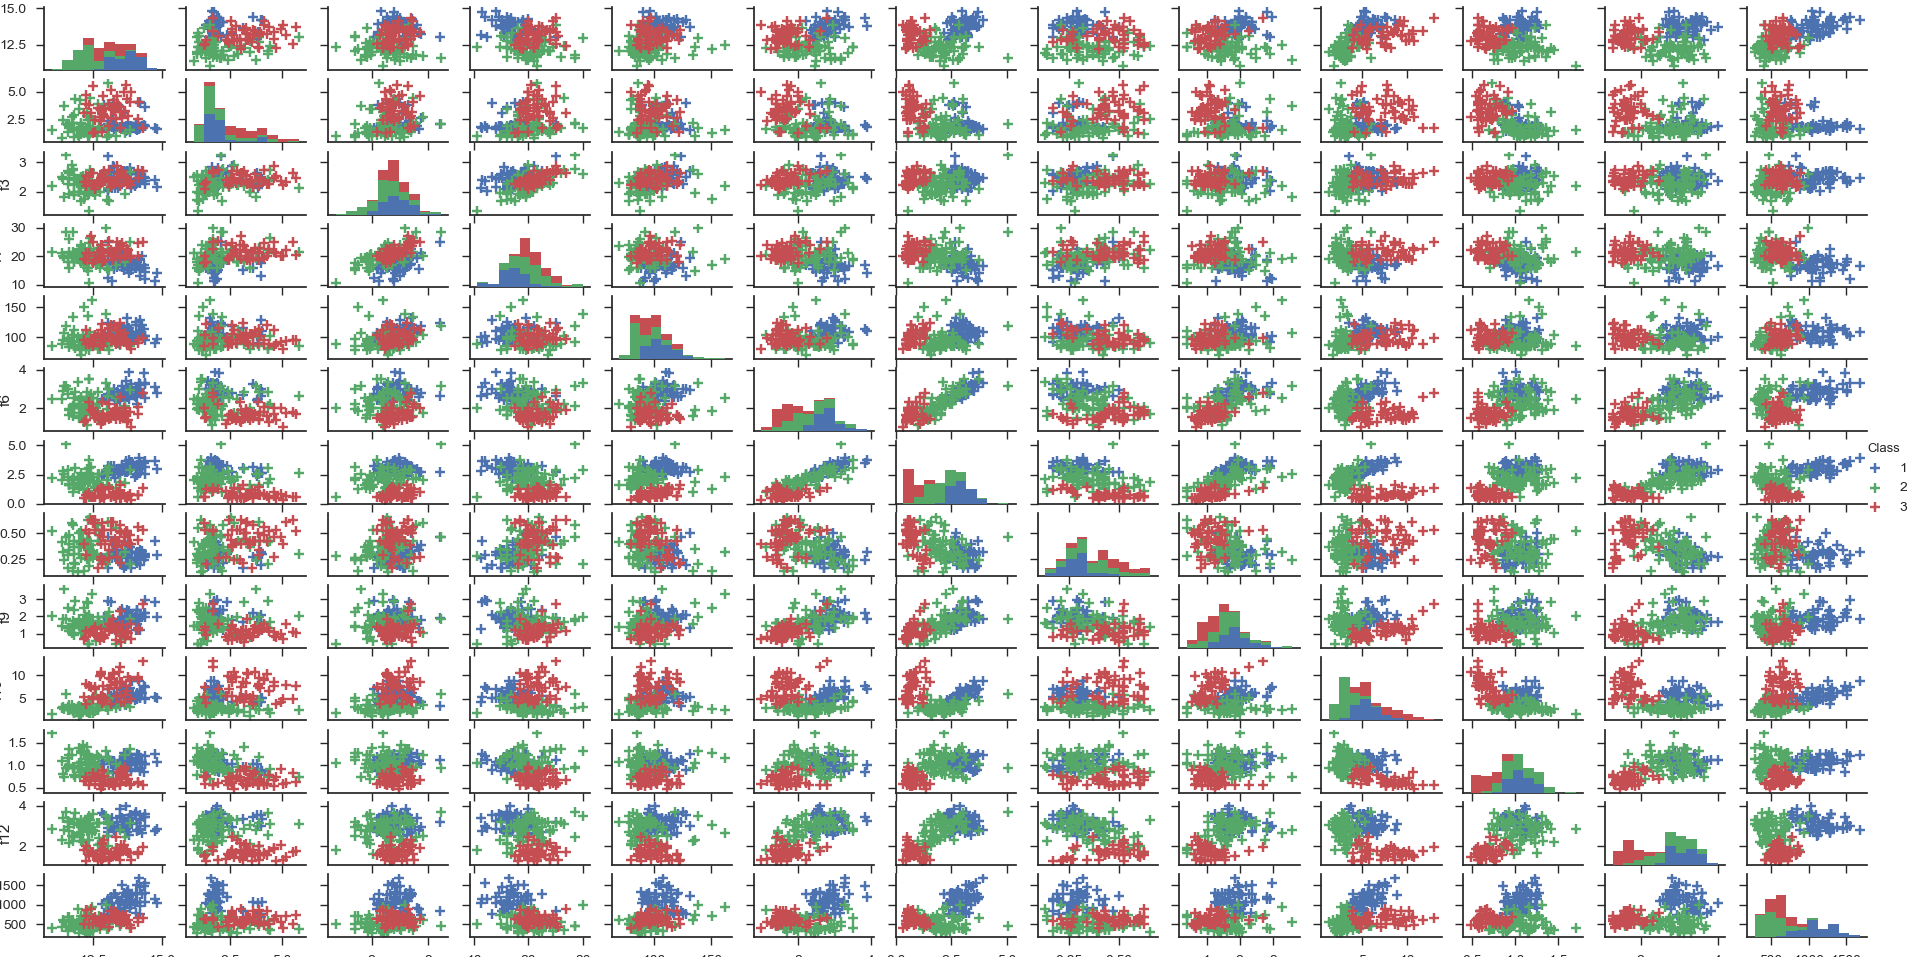
\includegraphics[width=1\textwidth]{dsWineCombined.png}
\caption{Rozkład cech dla zbioru Wine}
\end{figure}

\begin{figure}[H]
\centering
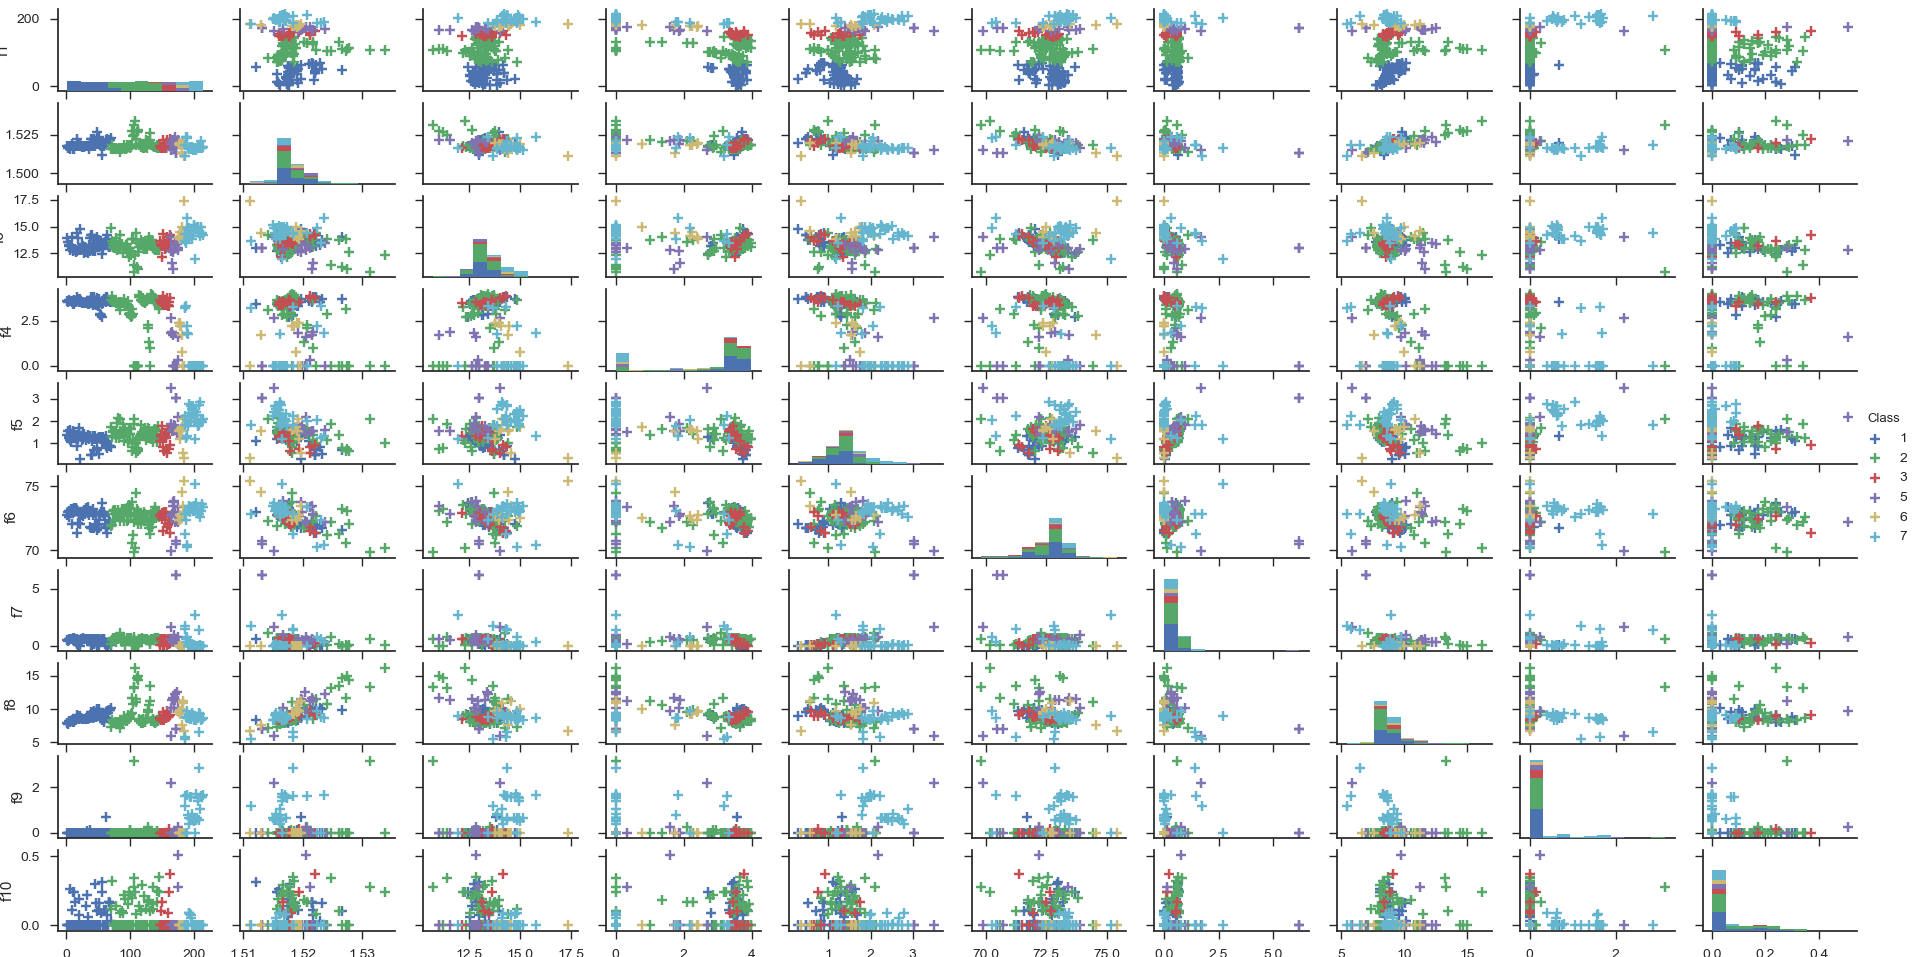
\includegraphics[width=1\textwidth]{dsGlassCombined.png}
\caption{Rozkład cech dla zbioru Glass}
\end{figure}

\begin{figure}[H]
\centering
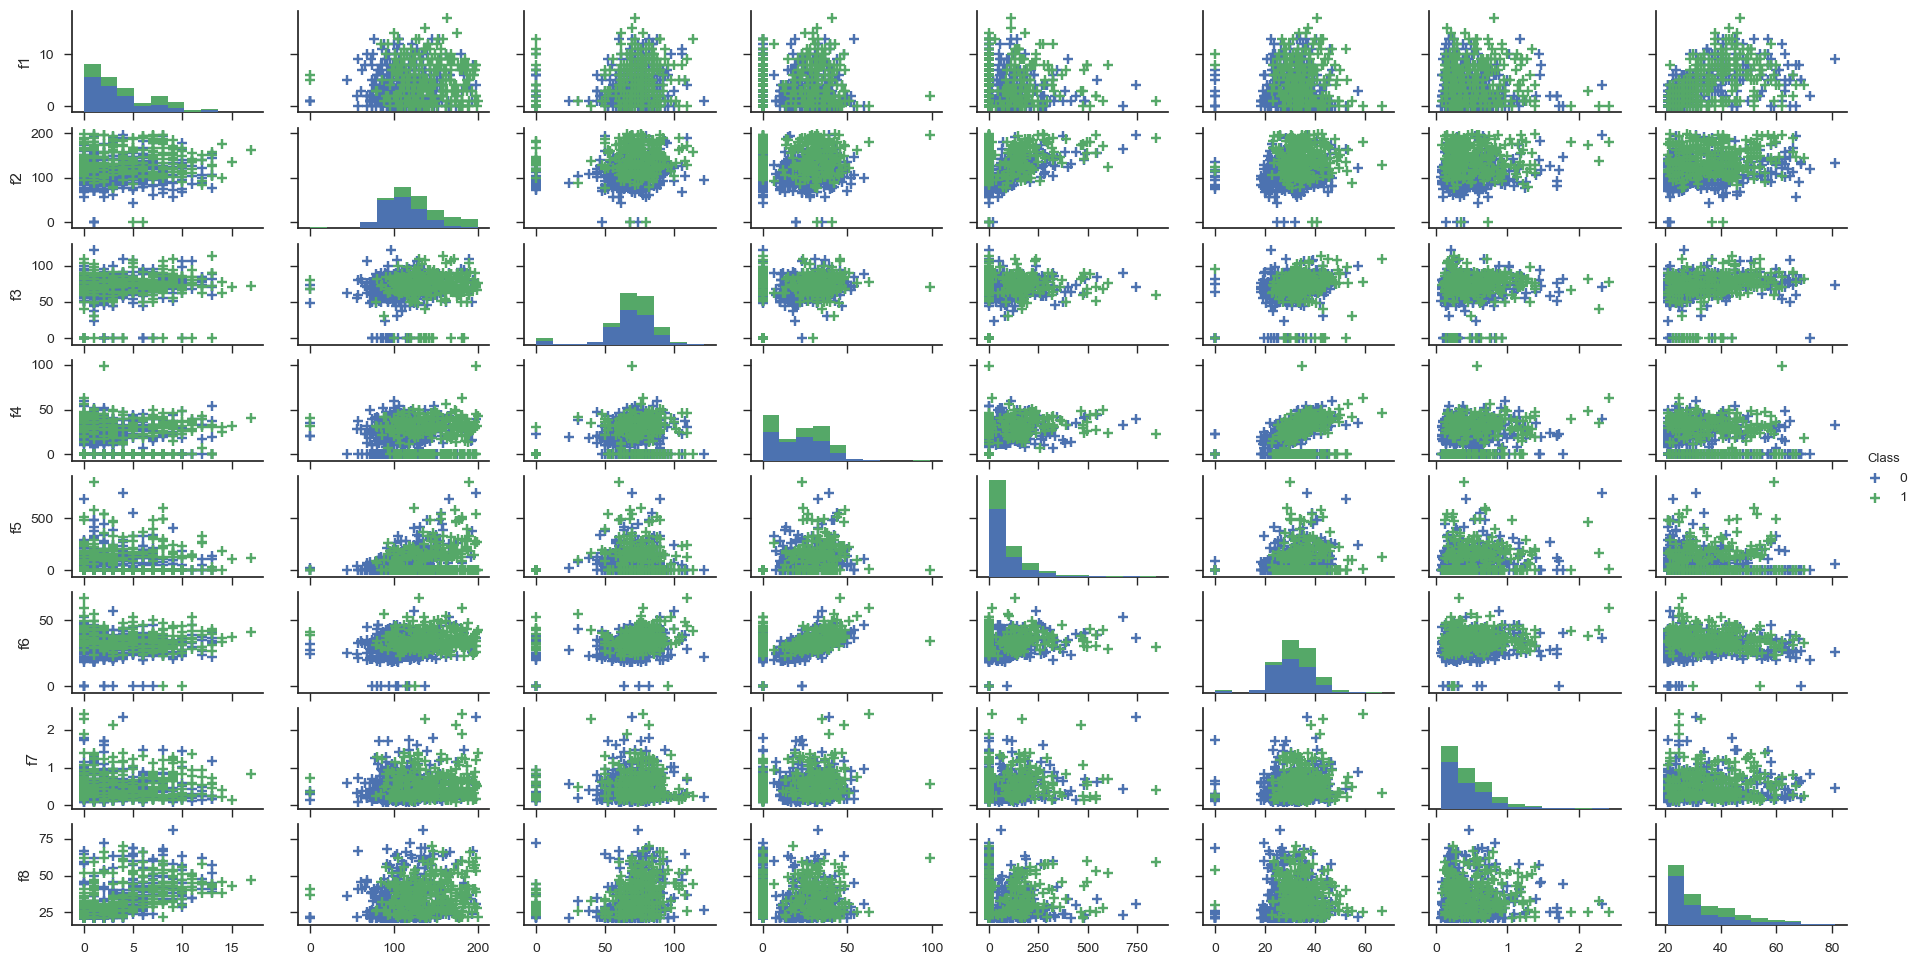
\includegraphics[width=1\textwidth]{dsDiabetesCombined.png}
\caption{Rozkład cech dla zbioru Diabetes}
\end{figure}

\begin{figure}[H]
\centering
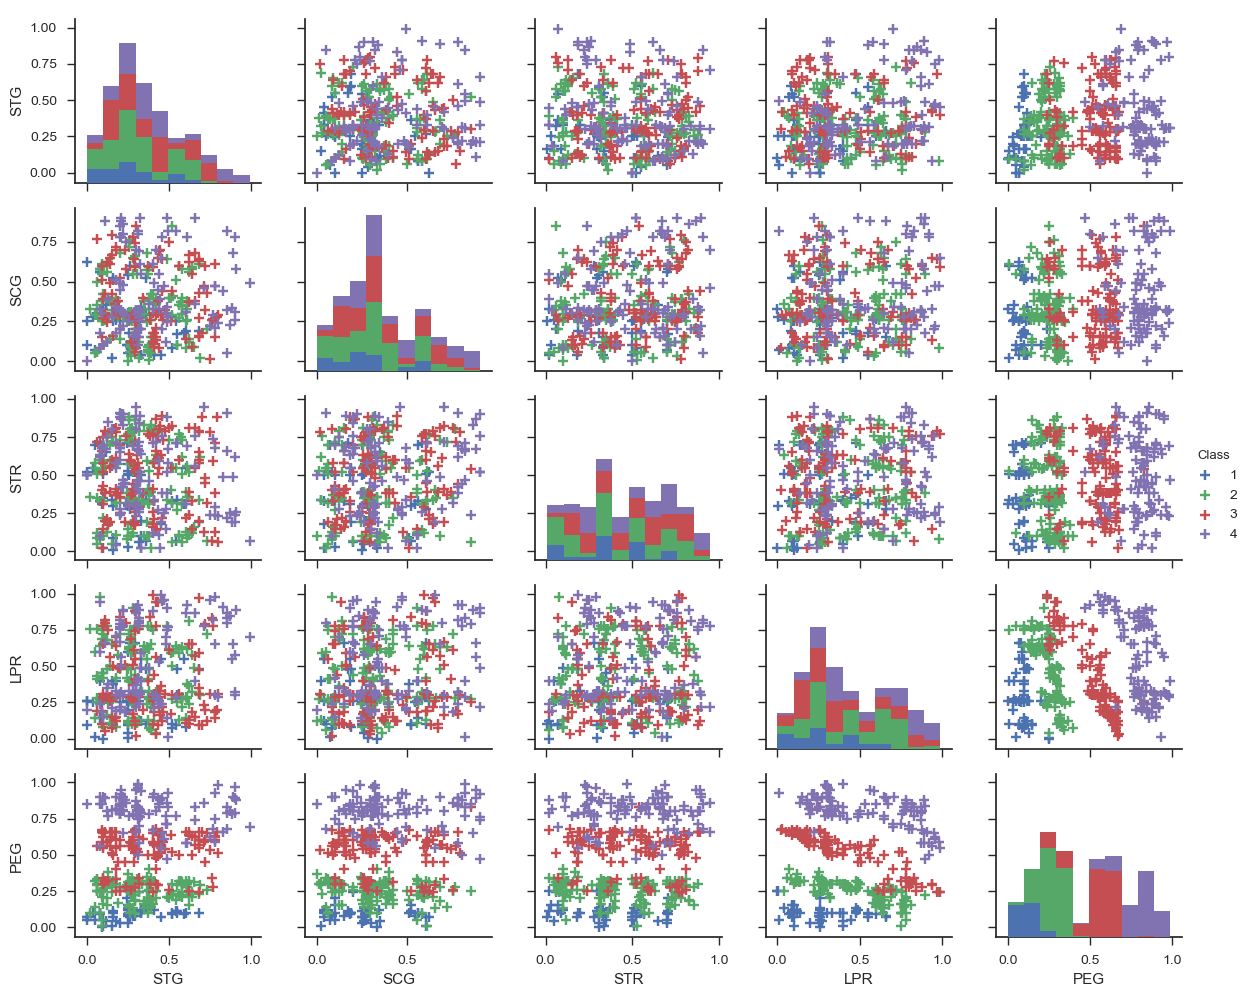
\includegraphics[width=1\textwidth]{dsKnowledgeCombined.png}
\caption{Rozkład cech dla zbioru Knowledge}
\end{figure}

\section{Normalizacja}
Wartości dla wszystkich zbiorów zostały znormalizowane, aby uniknąć przewagi jednego z atrybutów nad innymi. W przypadku instancji wine bez normalizacji wynik fscore wynosi 0.752, a w przypadku normalizacji danych wyniki wzrósł do 0.972.

\section{Wpływ doboru metryki na wyniki}

Dla każdego ze zbiorów zbadano wpływ doboru metryki na jakość klasyfikacji. Sposób głosowania dla tej próby zostanie ustawiony na \textit{squaredDistances}, dla 5 sąsiadów oraz rozmiarze kroswalidacji 5.\\
\begin{tabular}{ |p{2.5cm}||p{2.5cm}|p{2.5cm}|p{2.5cm}|p{2.5cm}| }
\hline
Metric &Accuracy & Precision & Recall & FScore \\
\hline
\multicolumn{5}{|c|}{Instanacja Wine}\\
\hline
euclidean & 0.955 & 0.959 & 0.955 & 0.955\\
manhattan & 0.972 & 0.973 & 0.972 & 0.972\\
\hline
\multicolumn{5}{|c|}{Instanacja Glass}\\ 
\hline
euclidean & 0.66 &, 0.672 & 0.668 & 0.665\\
manhattan & 0.682 & 0.684 & 0.682 & 0.677\\
\hline
\multicolumn{5}{|c|}{Instanacja Diabetes}\\  
\hline
euclidean & 0.74 & 0.651 & 0.567 & 0.606\\
manhattan & 0.742 & 0.655 & 0.552 & 0.599\\
\hline
\multicolumn{5}{|c|}{Instanacja Knowledge}\\  
\hline
euclidean & 0.813 & 0.826 & 0.813 & 0.811\\
manhattan & 0.848 & 0.854 & 0.848 & 0.848\\
\hline
\end{tabular}

\begin{figure}[H]
\centering
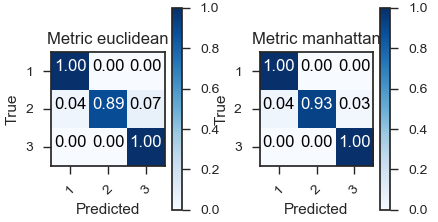
\includegraphics[width=1\textwidth]{MetricsWine.PNG}
\caption{Confusion Matrix dla zbioru Wine}
\end{figure}

\begin{figure}[H]
\centering
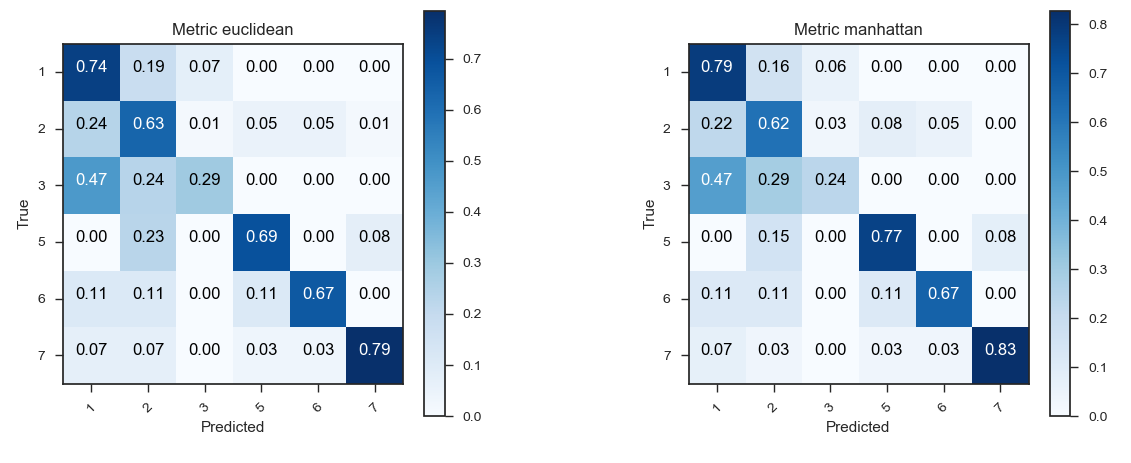
\includegraphics[width=1\textwidth]{MetricsGlass.PNG}
\caption{Confusion Matrix dla zbioru Glass}
\end{figure}

\begin{figure}[H]
\centering
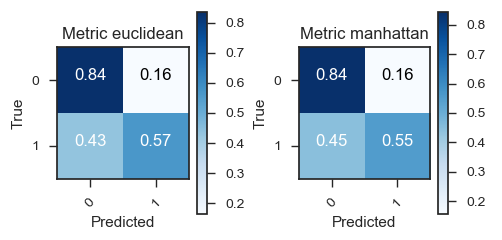
\includegraphics[width=1\textwidth]{MetricsDiabetes.PNG}
\caption{Confusion Matrix dla zbioru Diabetes}
\end{figure}

\begin{figure}[H]
\centering
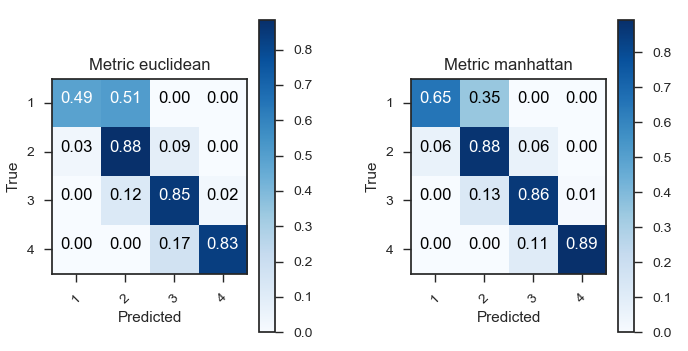
\includegraphics[width=1\textwidth]{MetricsKnowledge.PNG}
\caption{Confusion Matrix dla zbioru Knowledge}
\end{figure}

Dla większości badanych zbiorów metryka \textit{manhattan} daje lepsze rezultaty. Jedyny wyjątek stanowi zbiór \textit{Diabetes}, ale może to być spowodowane losowością w procesie kroswalidacji.

\section{Badanie sposobu głosowania}
Dla wszystkich badanych zbiorów przetestowane zostaną różne metody głosowania. Badanie zostanie przeprowadzone dla parametru k=5, metryce manhatan i rozmiarze kroswalidacji 5.

\begin{tabular}{ |p{3cm}||p{2cm}|p{2cm}|p{2cm}|p{2cm}| }
\hline
Voting & Accuracy & Precision & Recall & FScore \\
\hline
\hline
\multicolumn{5}{|c|}{Wine}\\
\hline
uniform & 0.966 & 0.968 & 0.966 & 0.966\\
distance & 0.972 & 0.973 & 0.972 & 0.972\\
squaredDistances & 0.972 & 0.973 & 0.972 & 0.972\\
\hline
\multicolumn{5}{|c|}{Glass}\\
\hline
uniform & 0.664 & 0.622 & 0.664 & 0.636\\
distance & 0.701 & 0.7 & 0.701 & 0.69\\
squaredDistances & 0.682 & 0.684 & 0.682 & 0.677\\
\hline
\multicolumn{5}{|c|}{Diabetes}\\
\hline
uniform & 0.75 & 0.671 & 0.556 & 0.608\\
distance & 0.747 & 0.664 & 0.56 & 0.607\\
squaredDistances & 0.742 & 0.655 & 0.552 & 0.599\\
\hline
\multicolumn{5}{|c|}{Knowledge}\\
\hline
uniform & 0.841 & 0.85 & 0.841 & 0.84\\
distance & 0.856 & 0.864 & 0.856 & 0.855\\
squaredDistances & 0.848 & 0.854 & 0.848 & 0.848\\
\hline
\end{tabular}

\begin{figure}[H]
\centering
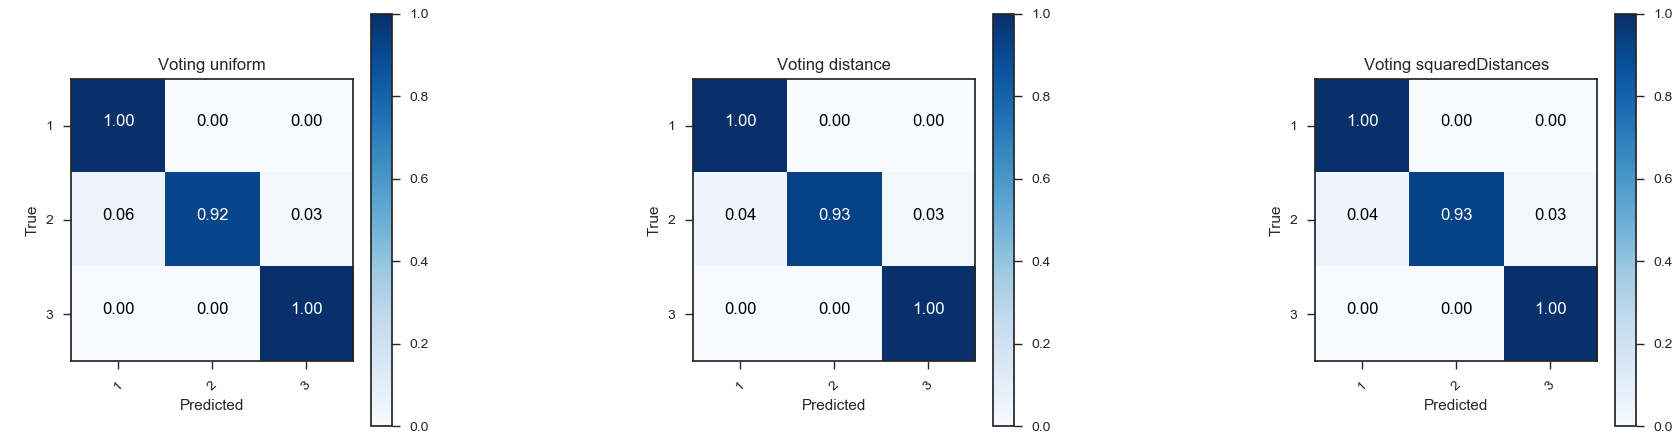
\includegraphics[width=1\textwidth]{VotingWine.PNG}
\caption{Confusion Matrix dla zbioru Wine}
\end{figure}

\begin{figure}[H]
\centering
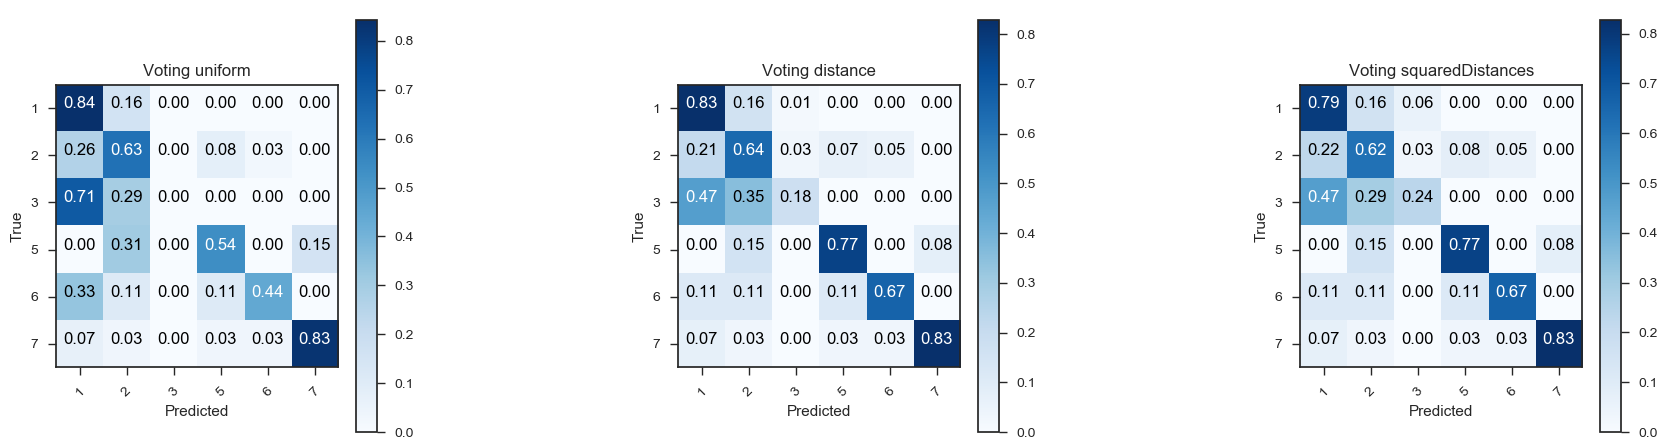
\includegraphics[width=1\textwidth]{VotingGlass.PNG}
\caption{Confusion Matrix dla zbioru Glass}
\end{figure}

\begin{figure}[H]
\centering
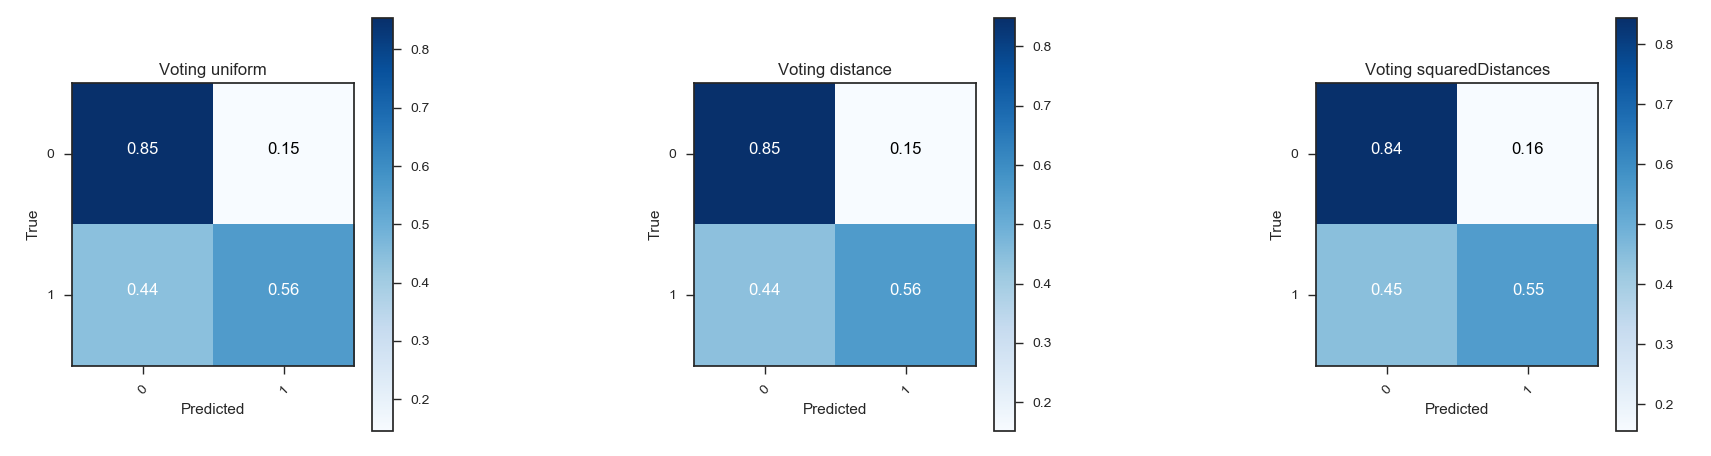
\includegraphics[width=1\textwidth]{VotingDiabetes.PNG}
\caption{Confusion Matrix dla zbioru Diabetes}
\end{figure}

\begin{figure}[H]
\centering
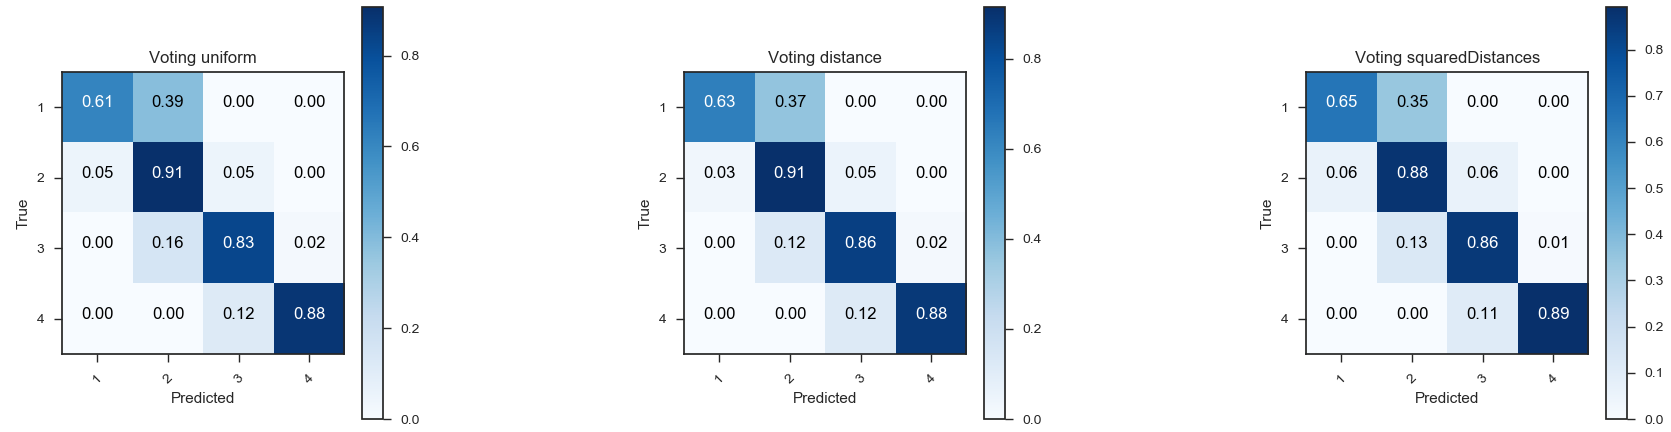
\includegraphics[width=1\textwidth]{VotingKnowledge.PNG}
\caption{Confusion Matrix dla zbioru Knowledge}
\end{figure}

Głosowanie na podstawie dystansu zwykle daje najlepsze wyniki. Metoda \textit{uniform} w przypadku zbioru \textit{Glass} sprawiła, że do jednej z klas nie został zakwalifikowany żaden obiekt. Metody bazujące na dystansie potrafią skorygować sytuacje, gdy liczba obiektów w danej klasie nie jest zbyt duża.

\section{Badanie parametru k}
Dla sposobu pomiaru odległości \textit{uniform} i \textit{distance} zbadano wpływ parametru k dla wszystkich zbiorów przy metodzie liczenia odległości \textit{manhatan} i rozmiarze kroswalidacji 5.

 \begin{tabular}{ |p{2.5cm}||p{2.5cm}|p{2.5cm}|p{2.5cm}|p{2.5cm}| }
\hline
\multicolumn{5}{|c|}{Metoda głosowania uniform}\\
\hline
k & Accuracy & Precision & Recall & FScore \\
\hline
\multicolumn{5}{|c|}{Wine}\\
\hline
2 & 0.955 & 0.958 & 0.955 & 0.955\\
3 & 0.961 & 0.963 & 0.961 & 0.96\\
4 & 0.972 & 0.974 & 0.972 & 0.972\\
5 & 0.966 & 0.968 & 0.966 & 0.966\\
7 & 0.955 & 0.957 & 0.955 & 0.955\\
10 & 0.978 & 0.979 & 0.978 & 0.978\\
15 & 0.961 & 0.963 & 0.961 & 0.96\\
20 & 0.961 & 0.963 & 0.961 & 0.96\\
50 & 0.955 & 0.959 & 0.955 & 0.955\\
\hline
\multicolumn{5}{|c|}{Glass}\\
\hline
2 & 0.626 & 0.637 & 0.626 & 0.628\\
3 & 0.673 & 0.685 & 0.673 & 0.672\\
4 & 0.659 & 0.66 & 0.659 & 0.652\\
5 & 0.701 & 0.7 & 0.701 & 0.69\\
7 & 0.692 & 0.699 & 0.692 & 0.679\\
10 & 0.673 & 0.704 & 0.673 & 0.649\\
15 & 0.664 & 0.702 & 0.664 & 0.639\\
20 & 0.64 & 0.593 & 0.64 & 0.604\\
50 & 0.631 & 0.586 & 0.631 & 0.582\\
\hline
\multicolumn{5}{|c|}{Diabetes}\\
\hline
2 & 0.72 & 0.699 & 0.347 & 0.464\\
3 & 0.727 & 0.626 & 0.537 & 0.578\\
4 & 0.728 & 0.677 & 0.422 & 0.52\\
5 & 0.75 & 0.671 & 0.556 & 0.608\\
7 & 0.732 & 0.657 & 0.485 & 0.558\\
10 & 0.741 & 0.723 & 0.418 & 0.53\\
15 & 0.758 & 0.716 & 0.507 & 0.594\\
20 & 0.758 & 0.741 & 0.47 & 0.575\\
50 & 0.751 & 0.794 & 0.388 & 0.521\\
\hline
\multicolumn{5}{|c|}{Knowledge}\\
\hline
2 & 0.774 & 0.794 & 0.774 & 0.777\\
3 & 0.841 & 0.847 & 0.841 & 0.841\\
4 & 0.821 & 0.833 & 0.821 & 0.822\\
5 & 0.841 & 0.85 & 0.841 & 0.84\\
7 & 0.851 & 0.864 & 0.851 & 0.849\\
10 & 0.836 & 0.852 & 0.836 & 0.834\\
15 & 0.851 & 0.872 & 0.851 & 0.848\\
20 & 0.843 & 0.872 & 0.843 & 0.84\\
50 & 0.751 & 0.805 & 0.751 & 0.738\\
\hline
\end{tabular}
\vspace{5cm}

\begin{tabular}{ |p{2.5cm}||p{2.5cm}|p{2.5cm}|p{2.5cm}|p{2.5cm}| }
\hline
\multicolumn{5}{|c|}{Metoda głosowania distance}\\
\hline
k & Accuracy & Precision & Recall & FScore \\
\hline
\multicolumn{5}{|c|}{Wine}\\
\hline
2 & 0.944 & 0.949 & 0.944 & 0.943\\
3 & 0.961 & 0.963 & 0.961 & 0.96\\
4 & 0.955 & 0.958 & 0.955 & 0.955\\
5 & 0.972 & 0.973 & 0.972 & 0.972\\
7 & 0.955 & 0.957 & 0.955 & 0.955\\
10 & 0.966 & 0.968 & 0.966 & 0.966\\
15 & 0.961 & 0.963 & 0.961 & 0.96\\
20 & 0.966 & 0.968 & 0.966 & 0.966\\
50 & 0.966 & 0.968 & 0.966 & 0.966\\
\hline
\multicolumn{5}{|c|}{Glass}\\
\hline
2 & 0.626 & 0.637 & 0.626 & 0.628\\
3 & 0.673 & 0.685 & 0.673 & 0.672\\
4 & 0.659 & 0.66 & 0.659 & 0.652\\
5 & 0.701 & 0.7 & 0.701 & 0.69\\
7 & 0.692 & 0.699 & 0.692 & 0.679\\
10 & 0.673 & 0.704 & 0.673 & 0.649\\
15 & 0.664 & 0.702 & 0.664 & 0.639\\
20 & 0.64 & 0.593 & 0.64 & 0.604\\
50 & 0.631 & 0.586 & 0.631 & 0.582\\
\hline
\multicolumn{5}{|c|}{Diabetes}\\
\hline
2 & 0.704 & 0.586 & 0.522 & 0.552\\
3 & 0.72 & 0.614 & 0.534 & 0.571\\
4 & 0.725 & 0.624 & 0.534 & 0.575\\
5 & 0.747 & 0.664 & 0.56 & 0.607\\
7 & 0.73 & 0.649 & 0.496 & 0.562\\
10 & 0.75 & 0.692 & 0.511 & 0.588\\
15 & 0.762 & 0.725 & 0.511 & 0.6\\
20 & 0.758 & 0.718 & 0.504 & 0.592\\
50 & 0.755 & 0.767 & 0.429 & 0.55\\
\hline
\multicolumn{5}{|c|}{Knowledge}\\
\hline
2 & 0.801 & 0.804 & 0.801 & 0.802\\
3 & 0.851 & 0.857 & 0.851 & 0.851\\
4 & 0.843 & 0.85 & 0.843 & 0.843\\
5 & 0.856 & 0.864 & 0.856 & 0.855\\
7 & 0.858 & 0.868 & 0.858 & 0.857\\
10 & 0.878 & 0.893 & 0.878 & 0.876\\
15 & 0.871 & 0.887 & 0.871 & 0.869\\
20 & 0.858 & 0.884 & 0.858 & 0.855\\
50 & 0.781 & 0.827 & 0.781 & 0.77\\
\hline
\end{tabular}
\vspace{5cm}

Współczynnik k w przypadku metody głosowania \textit{uniform} powinien być dobierany w taki sposób, aby nie było możliwości dopasowania wektor do takiej samej ilości reprezentantów innych klas. W przypadku metod bazujących na odległości nie ma to aż takiego znaczenia.

\section{Badanie rozmiaru kroswalidacji}
Dla każdego z badanych zbiorów zbadano jak ilość podziałów (a co z tym się wiąże wielkość ciągu uczącego) wpływa na jakość klasyfikacji. Zaimplementowana została kroswalidacja stratyfikowana. Pozostałe parametry zostały ustawione następująco: k=5, metryka="manhatan", sposób głosowania="distance".

\begin{tabular}{ |p{2.5cm}||p{2.5cm}|p{2.5cm}|p{2.5cm}|p{2.5cm}| }
\hline
Folds & Accuracy & Precision & Recall & FScore \\
\hline
\hline
\multicolumn{5}{|c|}{Wine}\\
\hline
2 & 0.944 & 0.949 & 0.944 & 0.943\\
3 & 0.961 & 0.964 & 0.961 & 0.96\\
4 & 0.972 & 0.973 & 0.972 & 0.972\\
5 & 0.972 & 0.973 & 0.972 & 0.972\\
6 & 0.966 & 0.968 & 0.966 & 0.966\\
7 & 0.966 & 0.968 & 0.966 & 0.966\\
8 & 0.972 & 0.973 & 0.972 & 0.972\\
9 & 0.972 & 0.973 & 0.972 & 0.972\\
10 & 0.972 & 0.973 & 0.972 & 0.972\\
\hline
\multicolumn{5}{|c|}{Glass}\\
\hline
2 & 0.593 & 0.57 & 0.593 & 0.575\\
3 & 0.636 & 0.617 & 0.636 & 0.621\\
4 & 0.668 & 0.665 & 0.668 & 0.658\\
5 & 0.701 & 0.7 & 0.701 & 0.69\\
6 & 0.706 & 0.706 & 0.706 & 0.694\\
7 & 0.696 & 0.698 & 0.696 & 0.687\\
8 & 0.682 & 0.683 & 0.682 & 0.676\\
9 & 0.692 & 0.703 & 0.692 & 0.682\\
10 & 0.701 & 0.706 & 0.701 & 0.69\\
\hline
\multicolumn{5}{|c|}{Diabetes}\\
\hline
2 & 0.74 & 0.655 & 0.537 & 0.59\\
3 & 0.75 & 0.674 & 0.549 & 0.605\\
4 & 0.747 & 0.67 & 0.545 & 0.601\\
5 & 0.747 & 0.664 & 0.56 & 0.607\\
6 & 0.732 & 0.641 & 0.526 & 0.578\\
7 & 0.736 & 0.641 & 0.552 & 0.593\\
8 & 0.738 & 0.648 & 0.549 & 0.594\\
9 & 0.738 & 0.648 & 0.549 & 0.594\\
10 & 0.743 & 0.656 & 0.556 & 0.602\\
\hline
\multicolumn{5}{|c|}{Knowledge}\\
\hline
2 & 0.846 & 0.855 & 0.846 & 0.846\\
3 & 0.843 & 0.852 & 0.843 & 0.843\\
4 & 0.856 & 0.865 & 0.856 & 0.855\\
5 & 0.856 & 0.864 & 0.856 & 0.855\\
6 & 0.873 & 0.881 & 0.873 & 0.872\\
7 & 0.861 & 0.87 & 0.861 & 0.86\\
8 & 0.858 & 0.867 & 0.858 & 0.858\\
9 & 0.861 & 0.868 & 0.861 & 0.86\\
10 & 0.856 & 0.864 & 0.856 & 0.856\\
\hline
\end{tabular}

\section{Porównanie wyników między różnymi metodami klasyfikacji}
Dla każdego z algorytmów wybrane zostały optymalne parametry dla każdego ze zbiorów. Do porównania posły nam wyznacznik \textit{F-score}.

\begin{tabular}{ |p{2.5cm}||p{2.5cm}|p{2.5cm}|p{2.5cm}| }
\hline
Data Set & Bayes & C4.5 & knn \\
\hline
Wine & 0.957 & 0.932 & 0.972 \\
Glass & 0.646 & 0.691 & 0.690 \\
Diabetes & 0.748 & 0.816 & 0.608 \\
\hline
\end{tabular}

\begin{figure}[H]
\centering
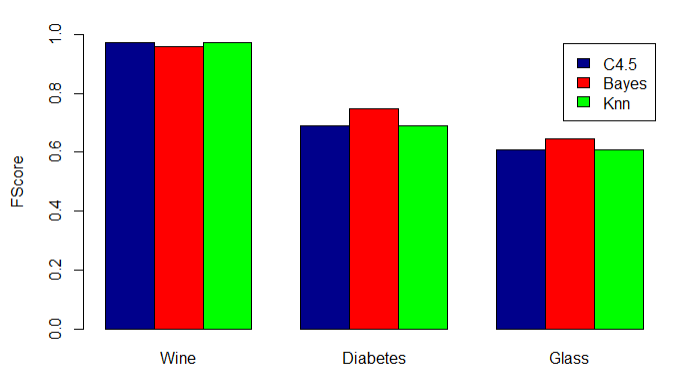
\includegraphics[width=1\textwidth]{Comparasion.PNG}
\caption{Porównanie działania algorytmów dla trzech zbiorów.}
\end{figure}

\section{Wnioski}
Mimo relatywnie prostego działania algorytm knn, daje dobre wyniki. Dla zbioru otrzymane wyniki są nawet lepsze niż dla pozostałych zbiorów. Dla dużych zbiorów dość szybko wzrasta czas potrzebny na selekcję najbliższych sąsiadów.
\end{document}
